\chapter{Theorie des graphes}
\section{Définitions et concept fondamental (graphe non orienté)}
\subsection{Définitions}
De façon conceptuelle, un graphe est formé par des sommets (Vertices en anglais) et des arêtes (Edges en anglais) 
qui relient les sommets entre-eux.

\begin{figure}[h]
\centering
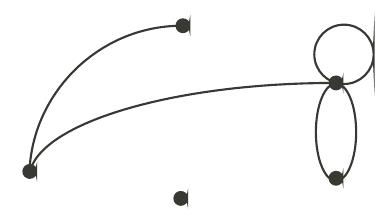
\includegraphics[width=0.5\linewidth]{images/graph}
\caption[Exemple d'un graphe]{Exemple d'un graphe}
\label{fig:graph}
\end{figure}

\subsection{Chaînes, chemain, circuit}

\subsection{Operations dans un graphe}

\subsection{Coupes}

\subsection{Isomorphisme d'un graphe}


\section{Arbres}
\subsection{Arbres et forêts}

\subsection{Circuits et ensembles de coupe}

\section{Graphe orienté}
\subsection{Définition}

\subsection{Arbres orienté}

\subsection{Graphe orienté acyclique}

\section{Matrices et espace vectoriel d'un graphe}
\subsection{Matrice associé d'un graphe}
\subsection{Matrice d'une coupe}
\subsection{Matrice  d'un circuit}
\subsection{Application: Stationary Linear Networks}
\subsection{Matrices over GF(2) and Vector Spaces of Graphs}

